% Options for packages loaded elsewhere
\PassOptionsToPackage{unicode}{hyperref}
\PassOptionsToPackage{hyphens}{url}
\PassOptionsToPackage{dvipsnames,svgnames,x11names}{xcolor}
%
\documentclass[
  letterpaper,
  DIV=11,
  numbers=noendperiod]{scrartcl}

\usepackage{amsmath,amssymb}
\usepackage{iftex}
\ifPDFTeX
  \usepackage[T1]{fontenc}
  \usepackage[utf8]{inputenc}
  \usepackage{textcomp} % provide euro and other symbols
\else % if luatex or xetex
  \usepackage{unicode-math}
  \defaultfontfeatures{Scale=MatchLowercase}
  \defaultfontfeatures[\rmfamily]{Ligatures=TeX,Scale=1}
\fi
\usepackage{lmodern}
\ifPDFTeX\else  
    % xetex/luatex font selection
\fi
% Use upquote if available, for straight quotes in verbatim environments
\IfFileExists{upquote.sty}{\usepackage{upquote}}{}
\IfFileExists{microtype.sty}{% use microtype if available
  \usepackage[]{microtype}
  \UseMicrotypeSet[protrusion]{basicmath} % disable protrusion for tt fonts
}{}
\makeatletter
\@ifundefined{KOMAClassName}{% if non-KOMA class
  \IfFileExists{parskip.sty}{%
    \usepackage{parskip}
  }{% else
    \setlength{\parindent}{0pt}
    \setlength{\parskip}{6pt plus 2pt minus 1pt}}
}{% if KOMA class
  \KOMAoptions{parskip=half}}
\makeatother
\usepackage{xcolor}
\setlength{\emergencystretch}{3em} % prevent overfull lines
\setcounter{secnumdepth}{5}
% Make \paragraph and \subparagraph free-standing
\ifx\paragraph\undefined\else
  \let\oldparagraph\paragraph
  \renewcommand{\paragraph}[1]{\oldparagraph{#1}\mbox{}}
\fi
\ifx\subparagraph\undefined\else
  \let\oldsubparagraph\subparagraph
  \renewcommand{\subparagraph}[1]{\oldsubparagraph{#1}\mbox{}}
\fi

\usepackage{color}
\usepackage{fancyvrb}
\newcommand{\VerbBar}{|}
\newcommand{\VERB}{\Verb[commandchars=\\\{\}]}
\DefineVerbatimEnvironment{Highlighting}{Verbatim}{commandchars=\\\{\}}
% Add ',fontsize=\small' for more characters per line
\usepackage{framed}
\definecolor{shadecolor}{RGB}{241,243,245}
\newenvironment{Shaded}{\begin{snugshade}}{\end{snugshade}}
\newcommand{\AlertTok}[1]{\textcolor[rgb]{0.68,0.00,0.00}{#1}}
\newcommand{\AnnotationTok}[1]{\textcolor[rgb]{0.37,0.37,0.37}{#1}}
\newcommand{\AttributeTok}[1]{\textcolor[rgb]{0.40,0.45,0.13}{#1}}
\newcommand{\BaseNTok}[1]{\textcolor[rgb]{0.68,0.00,0.00}{#1}}
\newcommand{\BuiltInTok}[1]{\textcolor[rgb]{0.00,0.23,0.31}{#1}}
\newcommand{\CharTok}[1]{\textcolor[rgb]{0.13,0.47,0.30}{#1}}
\newcommand{\CommentTok}[1]{\textcolor[rgb]{0.37,0.37,0.37}{#1}}
\newcommand{\CommentVarTok}[1]{\textcolor[rgb]{0.37,0.37,0.37}{\textit{#1}}}
\newcommand{\ConstantTok}[1]{\textcolor[rgb]{0.56,0.35,0.01}{#1}}
\newcommand{\ControlFlowTok}[1]{\textcolor[rgb]{0.00,0.23,0.31}{#1}}
\newcommand{\DataTypeTok}[1]{\textcolor[rgb]{0.68,0.00,0.00}{#1}}
\newcommand{\DecValTok}[1]{\textcolor[rgb]{0.68,0.00,0.00}{#1}}
\newcommand{\DocumentationTok}[1]{\textcolor[rgb]{0.37,0.37,0.37}{\textit{#1}}}
\newcommand{\ErrorTok}[1]{\textcolor[rgb]{0.68,0.00,0.00}{#1}}
\newcommand{\ExtensionTok}[1]{\textcolor[rgb]{0.00,0.23,0.31}{#1}}
\newcommand{\FloatTok}[1]{\textcolor[rgb]{0.68,0.00,0.00}{#1}}
\newcommand{\FunctionTok}[1]{\textcolor[rgb]{0.28,0.35,0.67}{#1}}
\newcommand{\ImportTok}[1]{\textcolor[rgb]{0.00,0.46,0.62}{#1}}
\newcommand{\InformationTok}[1]{\textcolor[rgb]{0.37,0.37,0.37}{#1}}
\newcommand{\KeywordTok}[1]{\textcolor[rgb]{0.00,0.23,0.31}{#1}}
\newcommand{\NormalTok}[1]{\textcolor[rgb]{0.00,0.23,0.31}{#1}}
\newcommand{\OperatorTok}[1]{\textcolor[rgb]{0.37,0.37,0.37}{#1}}
\newcommand{\OtherTok}[1]{\textcolor[rgb]{0.00,0.23,0.31}{#1}}
\newcommand{\PreprocessorTok}[1]{\textcolor[rgb]{0.68,0.00,0.00}{#1}}
\newcommand{\RegionMarkerTok}[1]{\textcolor[rgb]{0.00,0.23,0.31}{#1}}
\newcommand{\SpecialCharTok}[1]{\textcolor[rgb]{0.37,0.37,0.37}{#1}}
\newcommand{\SpecialStringTok}[1]{\textcolor[rgb]{0.13,0.47,0.30}{#1}}
\newcommand{\StringTok}[1]{\textcolor[rgb]{0.13,0.47,0.30}{#1}}
\newcommand{\VariableTok}[1]{\textcolor[rgb]{0.07,0.07,0.07}{#1}}
\newcommand{\VerbatimStringTok}[1]{\textcolor[rgb]{0.13,0.47,0.30}{#1}}
\newcommand{\WarningTok}[1]{\textcolor[rgb]{0.37,0.37,0.37}{\textit{#1}}}

\providecommand{\tightlist}{%
  \setlength{\itemsep}{0pt}\setlength{\parskip}{0pt}}\usepackage{longtable,booktabs,array}
\usepackage{calc} % for calculating minipage widths
% Correct order of tables after \paragraph or \subparagraph
\usepackage{etoolbox}
\makeatletter
\patchcmd\longtable{\par}{\if@noskipsec\mbox{}\fi\par}{}{}
\makeatother
% Allow footnotes in longtable head/foot
\IfFileExists{footnotehyper.sty}{\usepackage{footnotehyper}}{\usepackage{footnote}}
\makesavenoteenv{longtable}
\usepackage{graphicx}
\makeatletter
\def\maxwidth{\ifdim\Gin@nat@width>\linewidth\linewidth\else\Gin@nat@width\fi}
\def\maxheight{\ifdim\Gin@nat@height>\textheight\textheight\else\Gin@nat@height\fi}
\makeatother
% Scale images if necessary, so that they will not overflow the page
% margins by default, and it is still possible to overwrite the defaults
% using explicit options in \includegraphics[width, height, ...]{}
\setkeys{Gin}{width=\maxwidth,height=\maxheight,keepaspectratio}
% Set default figure placement to htbp
\makeatletter
\def\fps@figure{htbp}
\makeatother
% definitions for citeproc citations
\NewDocumentCommand\citeproctext{}{}
\NewDocumentCommand\citeproc{mm}{%
  \begingroup\def\citeproctext{#2}\cite{#1}\endgroup}
\makeatletter
 % allow citations to break across lines
 \let\@cite@ofmt\@firstofone
 % avoid brackets around text for \cite:
 \def\@biblabel#1{}
 \def\@cite#1#2{{#1\if@tempswa , #2\fi}}
\makeatother
\newlength{\cslhangindent}
\setlength{\cslhangindent}{1.5em}
\newlength{\csllabelwidth}
\setlength{\csllabelwidth}{3em}
\newenvironment{CSLReferences}[2] % #1 hanging-indent, #2 entry-spacing
 {\begin{list}{}{%
  \setlength{\itemindent}{0pt}
  \setlength{\leftmargin}{0pt}
  \setlength{\parsep}{0pt}
  % turn on hanging indent if param 1 is 1
  \ifodd #1
   \setlength{\leftmargin}{\cslhangindent}
   \setlength{\itemindent}{-1\cslhangindent}
  \fi
  % set entry spacing
  \setlength{\itemsep}{#2\baselineskip}}}
 {\end{list}}
\usepackage{calc}
\newcommand{\CSLBlock}[1]{\hfill\break\parbox[t]{\linewidth}{\strut\ignorespaces#1\strut}}
\newcommand{\CSLLeftMargin}[1]{\parbox[t]{\csllabelwidth}{\strut#1\strut}}
\newcommand{\CSLRightInline}[1]{\parbox[t]{\linewidth - \csllabelwidth}{\strut#1\strut}}
\newcommand{\CSLIndent}[1]{\hspace{\cslhangindent}#1}

\KOMAoption{captions}{tableheading}
\makeatletter
\@ifpackageloaded{caption}{}{\usepackage{caption}}
\AtBeginDocument{%
\ifdefined\contentsname
  \renewcommand*\contentsname{Table of contents}
\else
  \newcommand\contentsname{Table of contents}
\fi
\ifdefined\listfigurename
  \renewcommand*\listfigurename{List of Figures}
\else
  \newcommand\listfigurename{List of Figures}
\fi
\ifdefined\listtablename
  \renewcommand*\listtablename{List of Tables}
\else
  \newcommand\listtablename{List of Tables}
\fi
\ifdefined\figurename
  \renewcommand*\figurename{Figure}
\else
  \newcommand\figurename{Figure}
\fi
\ifdefined\tablename
  \renewcommand*\tablename{Table}
\else
  \newcommand\tablename{Table}
\fi
}
\@ifpackageloaded{float}{}{\usepackage{float}}
\floatstyle{ruled}
\@ifundefined{c@chapter}{\newfloat{codelisting}{h}{lop}}{\newfloat{codelisting}{h}{lop}[chapter]}
\floatname{codelisting}{Listing}
\newcommand*\listoflistings{\listof{codelisting}{List of Listings}}
\makeatother
\makeatletter
\makeatother
\makeatletter
\@ifpackageloaded{caption}{}{\usepackage{caption}}
\@ifpackageloaded{subcaption}{}{\usepackage{subcaption}}
\makeatother
\ifLuaTeX
  \usepackage{selnolig}  % disable illegal ligatures
\fi
\usepackage{bookmark}

\IfFileExists{xurl.sty}{\usepackage{xurl}}{} % add URL line breaks if available
\urlstyle{same} % disable monospaced font for URLs
\hypersetup{
  pdftitle={Paper 2},
  pdfauthor={Gavin Crooks; Samarth Rajani},
  colorlinks=true,
  linkcolor={blue},
  filecolor={Maroon},
  citecolor={Blue},
  urlcolor={Blue},
  pdfcreator={LaTeX via pandoc}}

\title{Paper 2\thanks{Code and data are available at:
LINK.https://github.com/Crooksyyy/The-Effects-of-Social-Media , Original
data available
https://www.openicpsr.org/openicpsr/project/112081/version/V1/view}}
\author{Gavin Crooks \and Samarth Rajani}
\date{February 15, 2024}

\begin{document}
\maketitle
\begin{abstract}
First sentence. Second sentence. Third sentence. Fourth sentence.
\end{abstract}

\renewcommand*\contentsname{Table of contents}
{
\hypersetup{linkcolor=}
\setcounter{tocdepth}{3}
\tableofcontents
}
\section{Introduction}\label{intro}

Household income is defined as the gross income earned by all members in
a household above 15 years of age (SCOTT 2024). Over the years, it has
been debated whether household incomes at all affect one's affiliation
towards a political school of thought. It is a reasonable hypothesis to
assume a sort of relationship between income and voting either Democrat
or Republican, as both parties have different economic outlooks thereby
affecting incomes differently. Maybe higher income inequality polarizes
political leaning further. Therefore, it is in our best interests to
study whether the poor vote to improve their quality of life.

In `Income Inequality and Partisan Voting in the United States', Andrew
Gelman, Lane Kenworthy and Yu-Sung Su (Gelman, Kenworthy, and Su 2010)
make a case for higher earning Americans voting Republican, whereas Jeff
Madrick (\textbf{article?}) argues how working-class Americans voted
against their interests in voting Republican. Conflicting theories have
emerged, and we intend on tackling this issue at hand of whether
different income brackets tend to vote differently.

Our data has been obtained from `The Welfare Effects of Social Media'
(\textbf{paper?}) . Our code is supported by the following packages (R
Core Team 2022) (Wickham et al. 2019) (\textbf{her?}) (Xie 2023)

\section{Data}\label{sec-data}

\subsection{Data Introduction}\label{sec-dataintro}

The data used in this paper is from (cite og paper). The data used in
the paper is extremely complicated as it combines numerous data sets to
complete their analysis. In this paper, we wanted to simplify the data
to determine if their paper had underlying biases within the data. To do
this we focused on one of their eleven data sets, baseline dataset as it
was the most comprehensive. This data was collected through a facebook
ad. The respondents answered a number of questions including questions
about income, ethnicity, family, political beliefs and political
following. THis is a very useful data set outside the scope of the
original paper as it can be analyzed to answer a number of questions.
The data set was cleaned to focus on respondents income, race and how
closely they follow politics. This provided a data set of approximately
6000 complete responses after removing unfinished responses. This was a
substantial decrease from the orignal 24000 responses in the data.

\subsection{Income Data}\label{sec-income_data}

The variable within the data was the income variable. The questionnaire
included a categorical value for the the household income of
respondents. The data can be visualized in (\textbf{figure1?}). This
graph illustrates that the least number of households make greater than
100,000 USD, below 20,000USD or preferred not to answer. This graph also
shows what the categorical option were for the respondents to the
questionnaire. (\textbf{figure1?}) closely resembles the expected
distribution of USA household income. As expected in any income
distribution the majority of responses fall within the average income
ranges of the USA, between 20,000USD and 100,000USD. These factors
indicate that the data set has an accurate representation of household
income.

\begin{figure}

\centering{

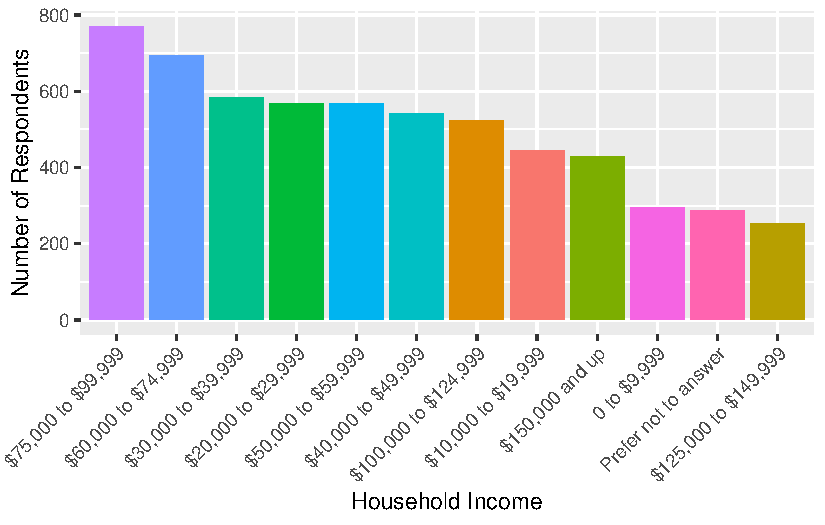
\includegraphics{paper_files/figure-pdf/fig-figure1-1.pdf}

}

\caption{\label{fig-figure1}Distribution of Income from Responses in a
facebook ad}

\end{figure}%

\subsection{Ethnicity Data}\label{sec-race_data}

The second question of the data that we have included in our analysis is
the ethnicity of the respondents. This again is a categorical variable,
that the individual self identifies their own ethnicity. The response
options included Asian or Pacific Islander, White / Caucasian, Hispanic,
Black or African American and other. (\textbf{race\_dist?}) shows the
percentage of respondents in each with the overwhelming majority of
responses being Caucasian at nearly 70\%. This is actually less than the
most recent estimates by the United States government which estimate
over 75\% of the population is Caucasian (cite us gov). The data also
has an over representation of Asian and Native Americans. This results
in an under representation of Hispanic and African American populations.

https://www.census.gov/quickfacts/fact/table/US/PST045222

\begin{longtable}[]{@{}lr@{}}

\caption{\label{tbl-race\_dist}Percentage of each Ethnicity from
Responses in a facebook ad}

\tabularnewline

\toprule\noalign{}
Ethnicity & Percentage of Responses \\
\midrule\noalign{}
\endhead
\bottomrule\noalign{}
\endlastfoot
American Indian or Alaskan Native & 0.7554138 \\
Asian or Pacific Islander & 13.5806614 \\
Black or African American & 6.0936713 \\
Hispanic & 8.0577472 \\
Other (please specify) & 2.5851939 \\
White / Caucasian & 68.9273124 \\

\end{longtable}

\subsection{Politics Data}\label{sec-pol_data}

The third variable in the data that is included in our analysis is a
variable of respondents self identifying how closely they follow
politics. This is another categorical variable measured as Not at all
closely, Somewhat closely, Rather closely and Very closely. This
variable faces many problems as this categorical scale is not consistent
across respondents. To be specific we mean someone who identifies as
someone who does follows Not at all closely can be following politics
more than someone who identifies as Somewhat closely. This is a
measurement issue within to the questions asked in the survey and all
self identifying variables in general. (\textbf{figure2?}) shows the
quantity of respondents in each group. The most common response is that
they follow somewhat closely and the other responses are relatively
even.

\begin{figure}

\centering{

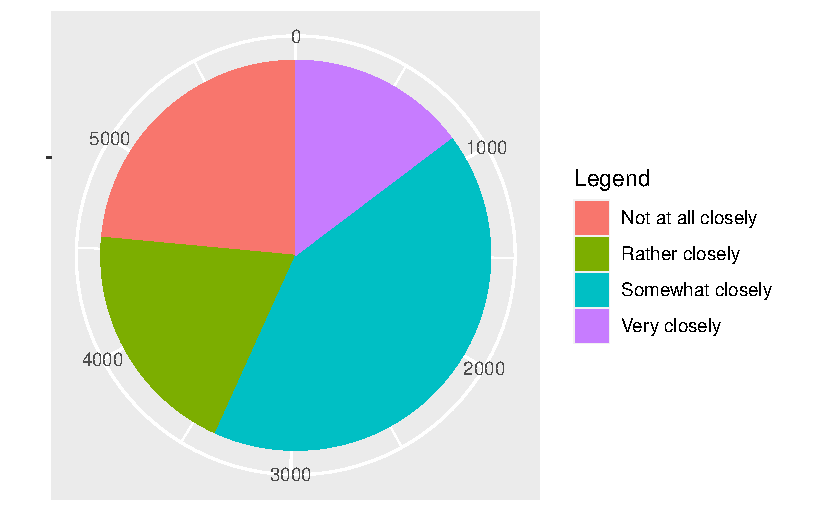
\includegraphics{paper_files/figure-pdf/fig-figure2-1.pdf}

}

\caption{\label{fig-figure2}How Closely People Follow Mr.Donald Trump
from Responses in a facebook ad}

\end{figure}%

\subsection{Missing Data}\label{sec-Missing_data}

\begin{figure}

\centering{

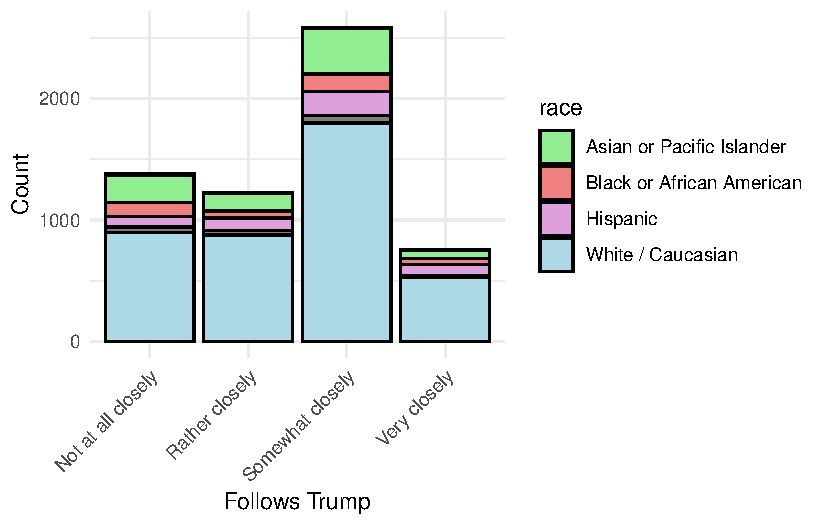
\includegraphics{paper_files/figure-pdf/fig-figure4-1.pdf}

}

\caption{\label{fig-figure4}Number of Respondents who follow Donald
Trump at different levels by Race}

\end{figure}%

\begin{figure}

\centering{

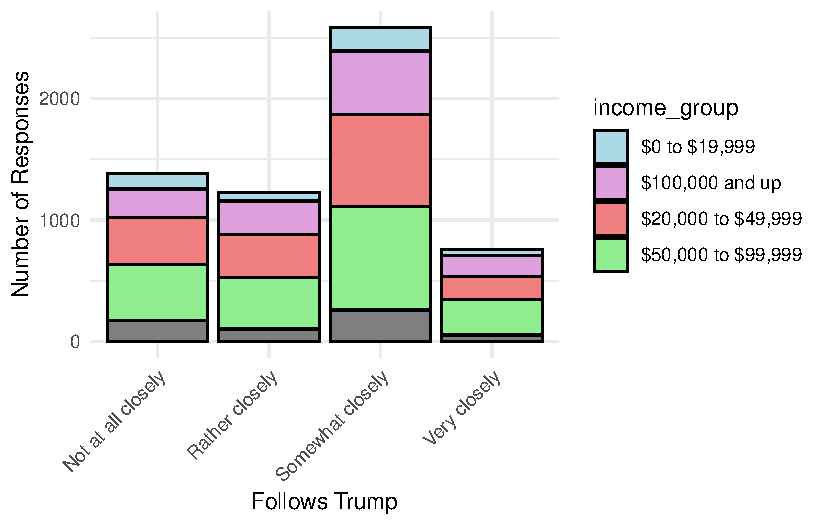
\includegraphics{paper_files/figure-pdf/fig-figure3-1.pdf}

}

\caption{\label{fig-figure3}Number of Respondents who follow Donald
Trump at different levels by Household Income}

\end{figure}%

\section{Results}\label{results}

\begin{Shaded}
\begin{Highlighting}[]
\CommentTok{\# Create a table of proportions}
\NormalTok{income\_follow\_table }\OtherTok{\textless{}{-}} \FunctionTok{table}\NormalTok{(cleaned\_data}\SpecialCharTok{$}\NormalTok{follow\_trump, cleaned\_data}\SpecialCharTok{$}\NormalTok{income\_group)}
\NormalTok{income\_proportions }\OtherTok{\textless{}{-}} \FunctionTok{prop.table}\NormalTok{(income\_follow\_table, }\AttributeTok{margin =} \DecValTok{1}\NormalTok{) }\SpecialCharTok{*} \DecValTok{100} 

\NormalTok{table1 }\OtherTok{\textless{}{-}} \FunctionTok{tibble}\NormalTok{(income\_proportions, }\FunctionTok{colnames}\NormalTok{(}\FunctionTok{c}\NormalTok{(}\StringTok{"Income Group"}\NormalTok{, }\StringTok{"Follows Trump"}\NormalTok{ )))}
\FunctionTok{show}\NormalTok{(table1)}
\end{Highlighting}
\end{Shaded}

\begin{verbatim}
# A tibble: 4 x 1
  income_proportions[,"$0 to $19,9~1 [,"$100,000 and up"] [,"$20,000 to $49,99~2
                               <dbl>                <dbl>                  <dbl>
1                               9.12                 16.9                   28.1
2                               5.86                 22.5                   29.0
3                               7.57                 20.2                   29.3
4                               6.73                 22.4                   25.3
# i abbreviated names: 1: income_proportions[,"$0 to $19,999"],
#   2: [,"$20,000 to $49,999"]
# i 1 more variable: income_proportions[4:5] <dbl>
\end{verbatim}

This papers goal was to identify if lower income household voted against
their own interest. To understand this relationship we used the variable
for how closely a respondent follows Mr.~Donald Trump as our measurement
of subscription to Republican ideas. Using this measurement, we
organized the proportion of individuals by income class to how closely
they follow Mr.~Donald Trump in Figure~\ref{fig-figure3}. This graph
shows that a proportional amount of each income class follows Mr.~Donald
Trump at similar levels across all income levels. Specifically, we mean
the percentage of individuals follow Mr.~Donald Trump at different
levels is the same no matter the income class. This means we can not
conclude that income class impacts how closely individuals follow
Mr.~Donald Trump, and therefor, cannot conclude that different income
levels subscribe to republican ideas more than the other.

To further our analysis we computed the same graph however organized by
race not income Figure~\ref{fig-figure4}. This resulted in a similar
result as race is proportional between all levels of following
Mr.~Donald Trump. Therefore, consistent across races at to following
republican rhetoric. Again, this means the same percentage of people
that follow Mr.~Donald Trump at different levels is the same for each
race. Obviously, this is more difficult to conclude for minorities as
their representation within the data set is so small as stated in
Section~\ref{sec-race_data}

Overall, the results of this analysis were inconclusive to measure how
income impacts individuals propensity to follow republican rhetoric.
There are many reasons this could be true and as stated in the
(\textbf{intro?}) there are multiple schools of thought previously
studies on the topic.

\section{Discussion}\label{discussion}

like to incluse variables like state etc data set too small/ incomplete
for that \#\# First discussion point \{\#sec-first-point\}

If my paper were 10 pages, then should be be at least 2.5 pages. The
discussion is a chance to show off what you know and what you learnt
from all this.

\subsection{Second discussion point}\label{second-discussion-point}

\subsection{Third discussion point}\label{third-discussion-point}

\subsection{Weaknesses and next steps}\label{weaknesses-and-next-steps}

Weaknesses and next steps should also be included.

\newpage

\appendix

\section*{Appendix}\label{appendix}
\addcontentsline{toc}{section}{Appendix}

\section{Additional data details}\label{additional-data-details}

\section{Model details}\label{sec-model-details}

\newpage

\section*{References}\label{references}
\addcontentsline{toc}{section}{References}

\phantomsection\label{refs}
\begin{CSLReferences}{1}{0}
\bibitem[\citeproctext]{ref-10.1257ux2faer.20190658}
Allcott, Hunt, Luca Braghieri, Sarah Eichmeyer, and Matthew Gentzkow.
2020. {``The Welfare Effects of Social Media.''} \emph{American Economic
Review}. \url{https://doi.org/10.1257/aer.20190658}.

\bibitem[\citeproctext]{ref-lane}
Gelman, Andrew, Lane Kenworthy, and Yu-Sung Su. 2010. {``Income
Inequality and Partisan Voting in the United States.''} \emph{Social
Science Quarterly}. {[}University of Texas Press, Wiley{]}.
\url{http://www.jstor.org/stable/42956457}.

\bibitem[\citeproctext]{ref-Madrick_2020}
Madrick, Jeff. 2020. {``Why the Working Class Votes Against Its Economic
Interests.''} \emph{The New York Times}, July.
\url{https://www.nytimes.com/2020/07/31/books/review/the-system-robert-reich-break-em-up-zephyr-teachout.html}.

\bibitem[\citeproctext]{ref-here}
Müller, Kirill. 2020. {``Here: A Simpler Way to Find Your Files.''}
\url{https://CRAN.R-project.org/package=here}.

\bibitem[\citeproctext]{ref-citeR}
R Core Team. 2022. \emph{R: A Language and Environment for Statistical
Computing}. Vienna, Austria: R Foundation for Statistical Computing.
\url{https://www.R-project.org/}.

\bibitem[\citeproctext]{ref-hhld}
SCOTT, MICHELLE P. 2024. {``Household Income.''} investopedia.
\url{https://www.investopedia.com/terms/h/household_income.asp}.

\bibitem[\citeproctext]{ref-tidy}
Wickham, Hadley, Mara Averick, Jennifer Bryan, Winston Chang, Lucy
D'Agostino McGowan, Romain François, Garrett Grolemund, et al. 2019.
{``Welcome to the {tidyverse}.''} \emph{Journal of Open Source
Software}. \url{https://doi.org/10.21105/joss.01686}.

\bibitem[\citeproctext]{ref-knitr}
Xie, Yihui. 2023. {``Knitr: A General-Purpose Package for Dynamic Report
Generation in r.''} \url{https://yihui.org/knitr/}.

\end{CSLReferences}



\end{document}
